\section{Running examples\label{section:background-running-examples}}

This section introduces the two running examples that will be used throughout the thesis. Section \ref{subsection:background-train-system} introduces a simple train control system. Section \ref{subsection:background-meeting-scheduler} introduces the meeting scheduler \cite{Feather:1997}.

\subsection{A simple train control system\label{subsection:background-train-system}}

A simplified train control system will be used as running example for illustrating concepts and techniques throughout this thesis. 

The system is composed of a software train controller, actuators for doors and train acceleration, sensors and passengers. Through the actuators, the software controller controls operations like starting or stopping the train, opening or closing doors, and so on. A safety goal requires train doors to remain closed while the train is moving. If the train is not moving and the passenger presses the alarm button, the controller must open the doors immediately. If the train is moving and the passenger presses the alarm button, the controller must stop the train first and then open the doors. 

Typical agent interactions for the latter case are depicted in Fig.~\ref{image:train-scenario-all-agents}. The precise semantics of such scenario will be made clear in the following sections.

\begin{figure}[H]\centering
\scalebox{0.75}{
  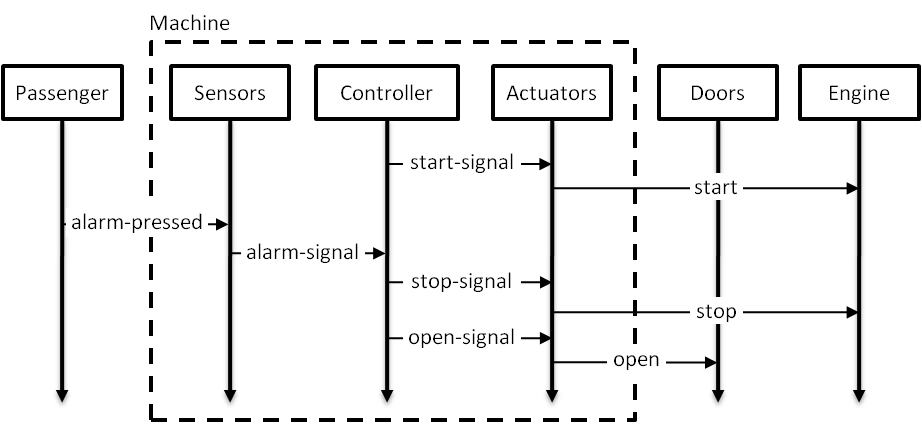
\includegraphics[trim=2mm 2mm 2mm 2mm, clip]{src/2-framework/images/train-scenario-all-agents}
}
\caption{A scenario illustrating a train system stopping in emergency when an alarm is pressed.\label{image:train-scenario-all-agents}}
\end{figure}

\subsection{The meeting scheduler\label{subsection:background-meeting-scheduler}}

For illustrating process models and associated techniques, we will focus on the following episode of a meeting scheduling process \cite{Feather:1997}. 

A meeting initiator issues a meeting request, specifying the expected participants and the date range within which the meeting should take place. The scheduler then sends an electronic invitation to each participant, requesting them to provide their constraints. 

A date conflict occurs when no date can be found that fits all participant constraints. In such case, the initiator may extend the date range or request some participants to weaken their constraints; a new scheduling cycle is then required. Otherwise, the meeting is planned at a date meeting all constraints.

A soft goal requires meetings to be scheduled as quickly as possible once initiated; another one requires the interactions with participants to be minimized. In the simplified version considered here, only two scheduling cycles are allowed; the meeting is automatically planned after that. In such case, we will asumme that the best date is chosen so as to maximize the number of attending participants. We also ignore features like meeting cancelations, meeting locations, and so on.

\begin{figure}[H]\centering
\scalebox{0.58}{
  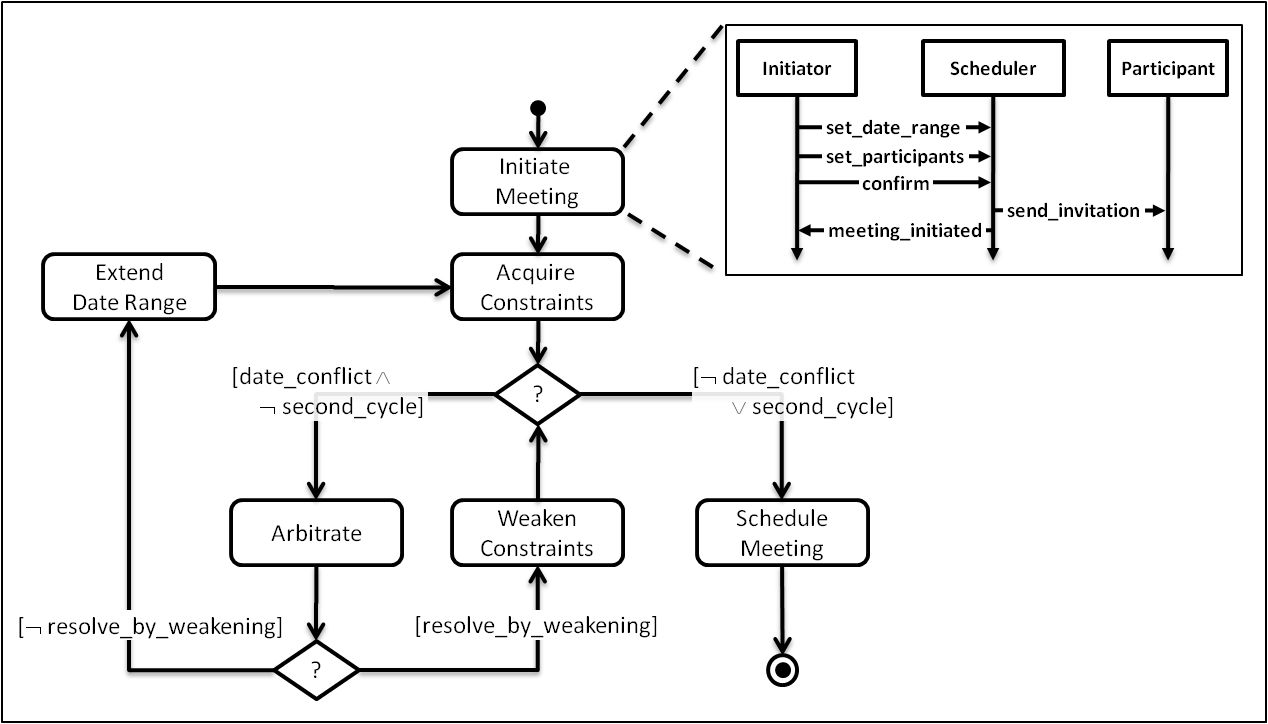
\includegraphics[trim=2mm 2mm 2mm 2mm, clip]{src/2-framework/images/scheduler-ghmsc}
}
\caption{A process model for a meeting scheduling process.\label{image:scheduler-ghmsc}}
\end{figure}

This meeting scheduling episode is illustrated in Fig.~\ref{image:scheduler-ghmsc}. The precise semantics of such model is detailed in Chapter \ref{chapter:deductive}.

